% \PassOptionsToPackage{showrules}{blurb}
% \PassOptionsToPackage{showframe}{blurb}
\documentclass[fleqn]{thesis}

% DOCUMENT
\usepackage{kantlipsum}

\graphicspath{{./ch3_creteil/img/}{./ch2_gridshell/img/}}


\begin{document}

	\part{My First Part}
		\chapter{Mon premier chapitre}
		\section{Une section}
		\kant[1-4]
		\section{Une deuxième section}
		\kant[1-2]
		\section{Une troisième section}
		\kant[1-2]
	
	\part{My Second Part}
		% \chapter{Mon premier chapitre}
		% \section{Une section}
		% \kant[1-20]
		% \section{Une deuxième section}
		% \kant[1-2]
		% \section{Une troisième section}
		% \kant[1-2]
		\cref{fig:twospread}


	\def\mycap{
		% \begin{textblock*}{5cm}(1cm,1cm)
		% 	\raggedright
		% 	\captionof{figure}{\LARGE\bfseries\color{white}sdsdksdmskdms\label{fig:twospread}}
		% \end{textblock*}
	}

\def\mycap{
	{\color{Tblue}\sffamily\bfseries\large\uppercase{Savill Building}}\\[0pt]
	{\sffamily\bfseries\uppercase{Gleen Howell Architects}}\\[8pt]
	{\color{gray}\sffamily\small The larch and oak structure is the end-result of much refinement, combining complex engineering and craft skills and is one of the few true shell roofs in existence.}}

	\clearpage
	% \begin{textblock*}{0.5\paperwidth}(0cm,0cm)
	% 	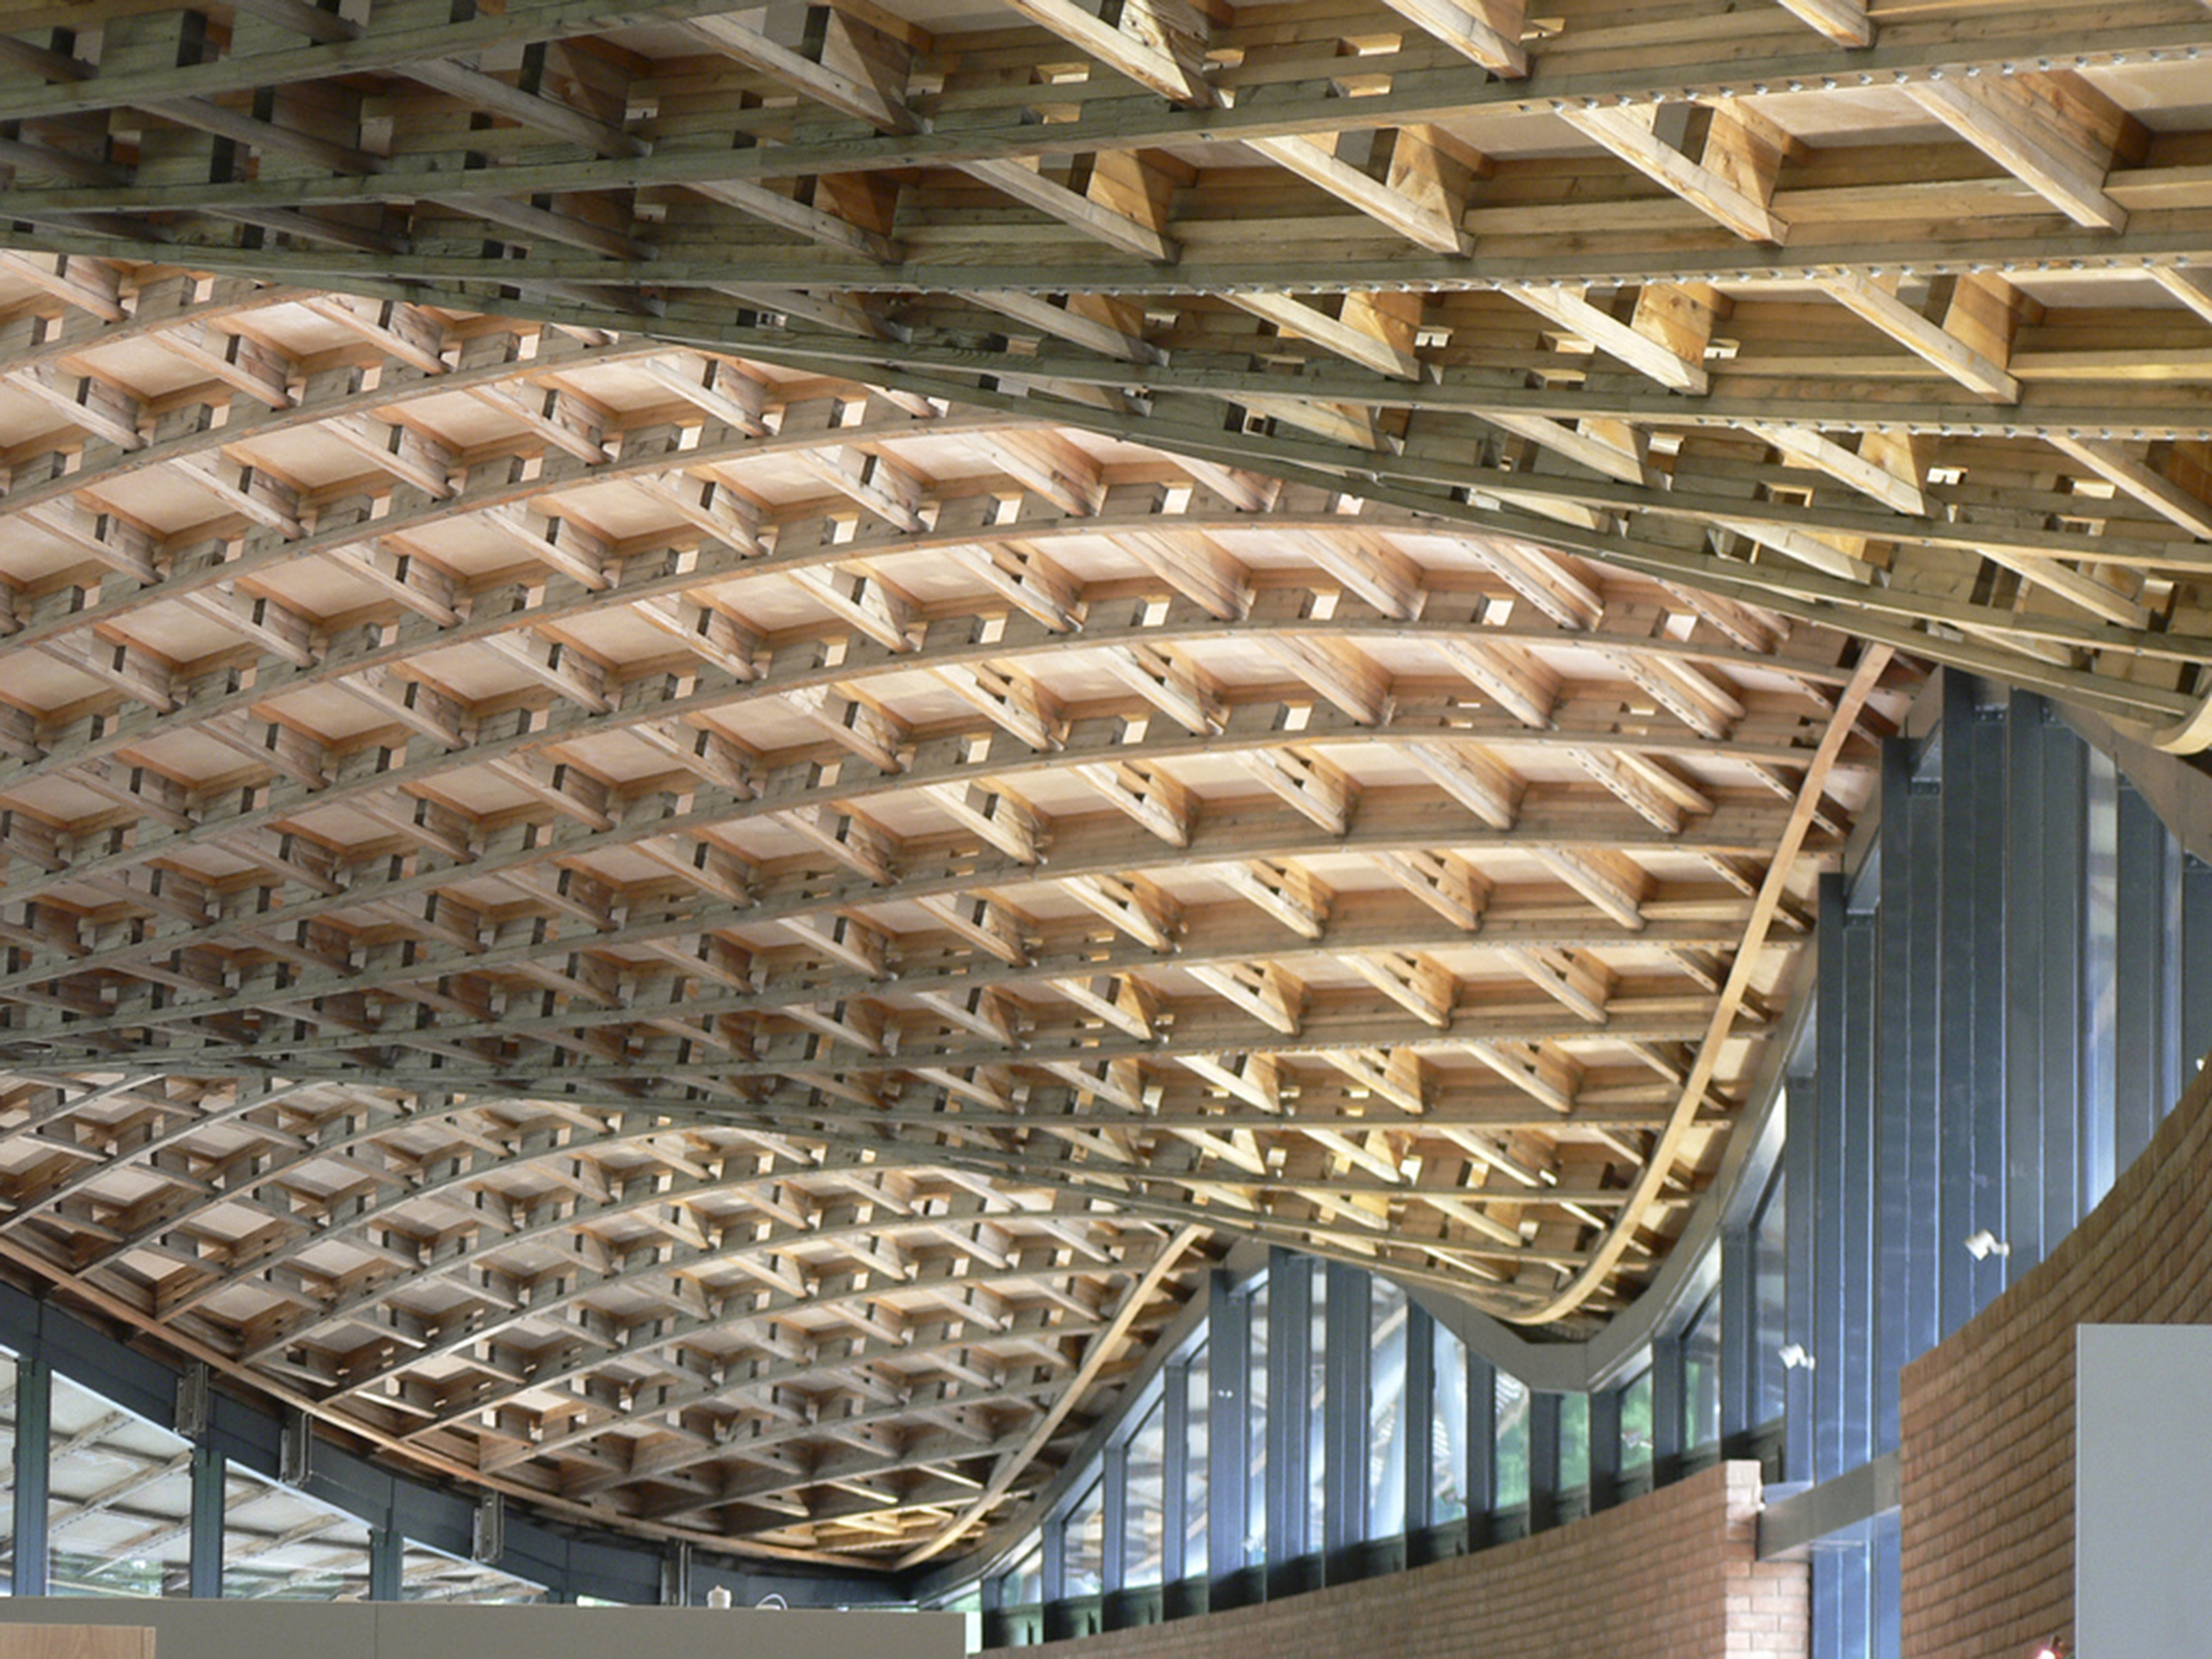
\includegraphics[width=0.5\paperwidth]{savill_b.jpg}
	% \end{textblock*}
	
	% full spread
	\cleartoleftpage
	\kant[1-2]	
	
	\begin{figure}[t]
		% (%) required at end of lines to prevent extra space
		\hrule
		%
		\begin{subfigure}[b]{\TwoMediaWidth}
			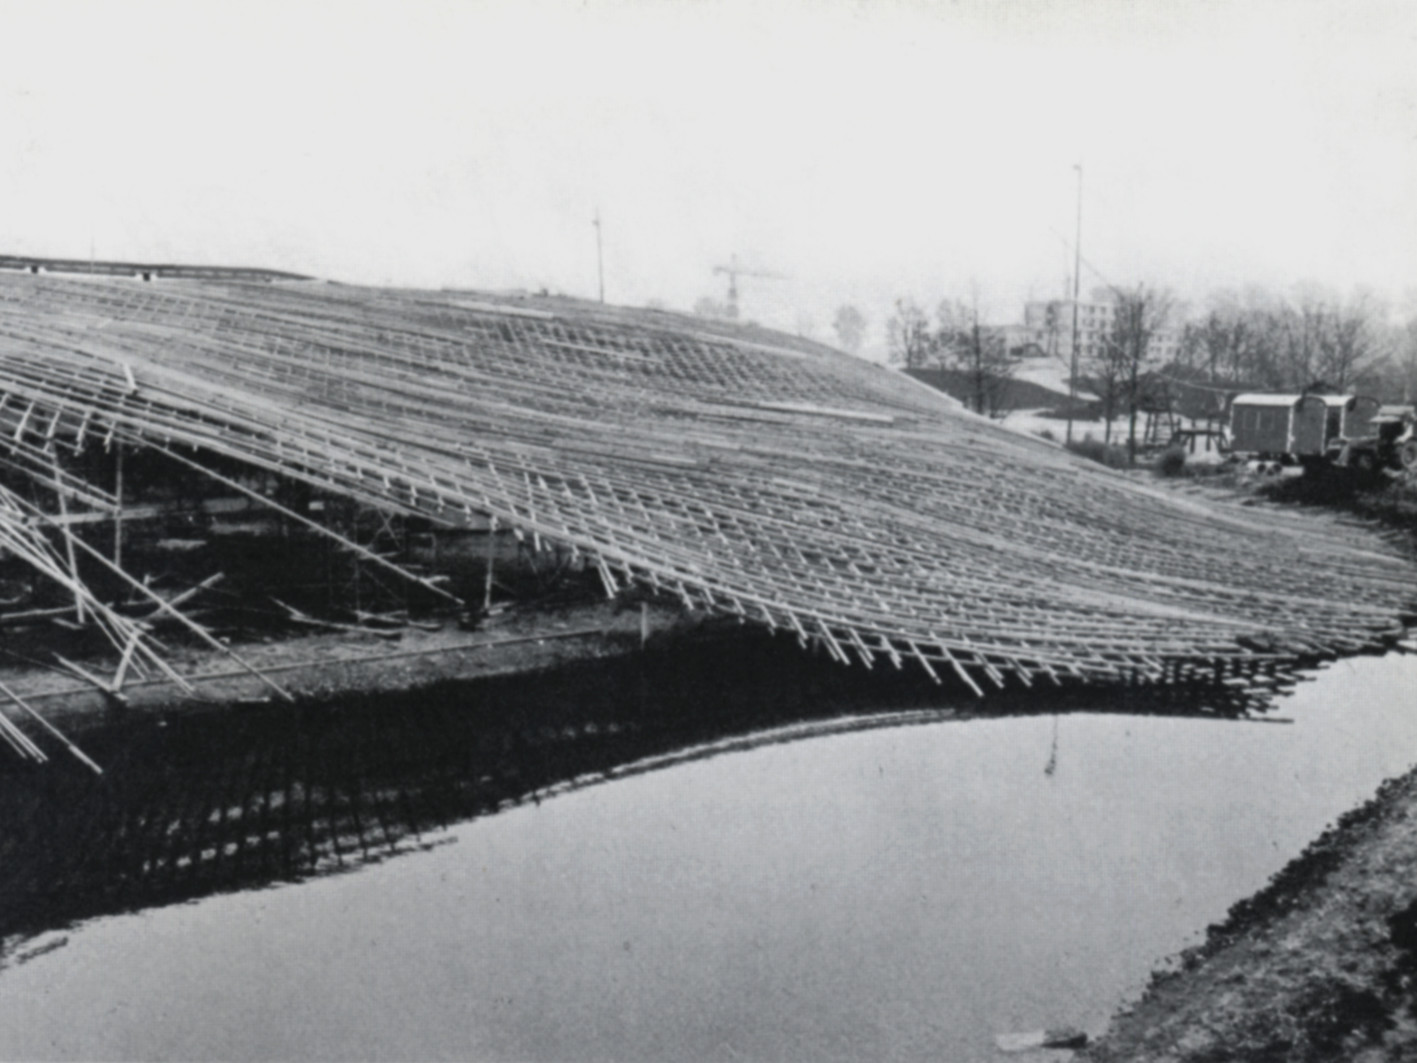
\includegraphics[width=\textwidth]{mannheim_erection_1.jpg}
			\caption{Almost flat grid}
			\label{fig:erec_1}
		\end{subfigure}%
		\hspace{\MediaGutterWidth}%
		\begin{subfigure}[b]{\TwoMediaWidth}
			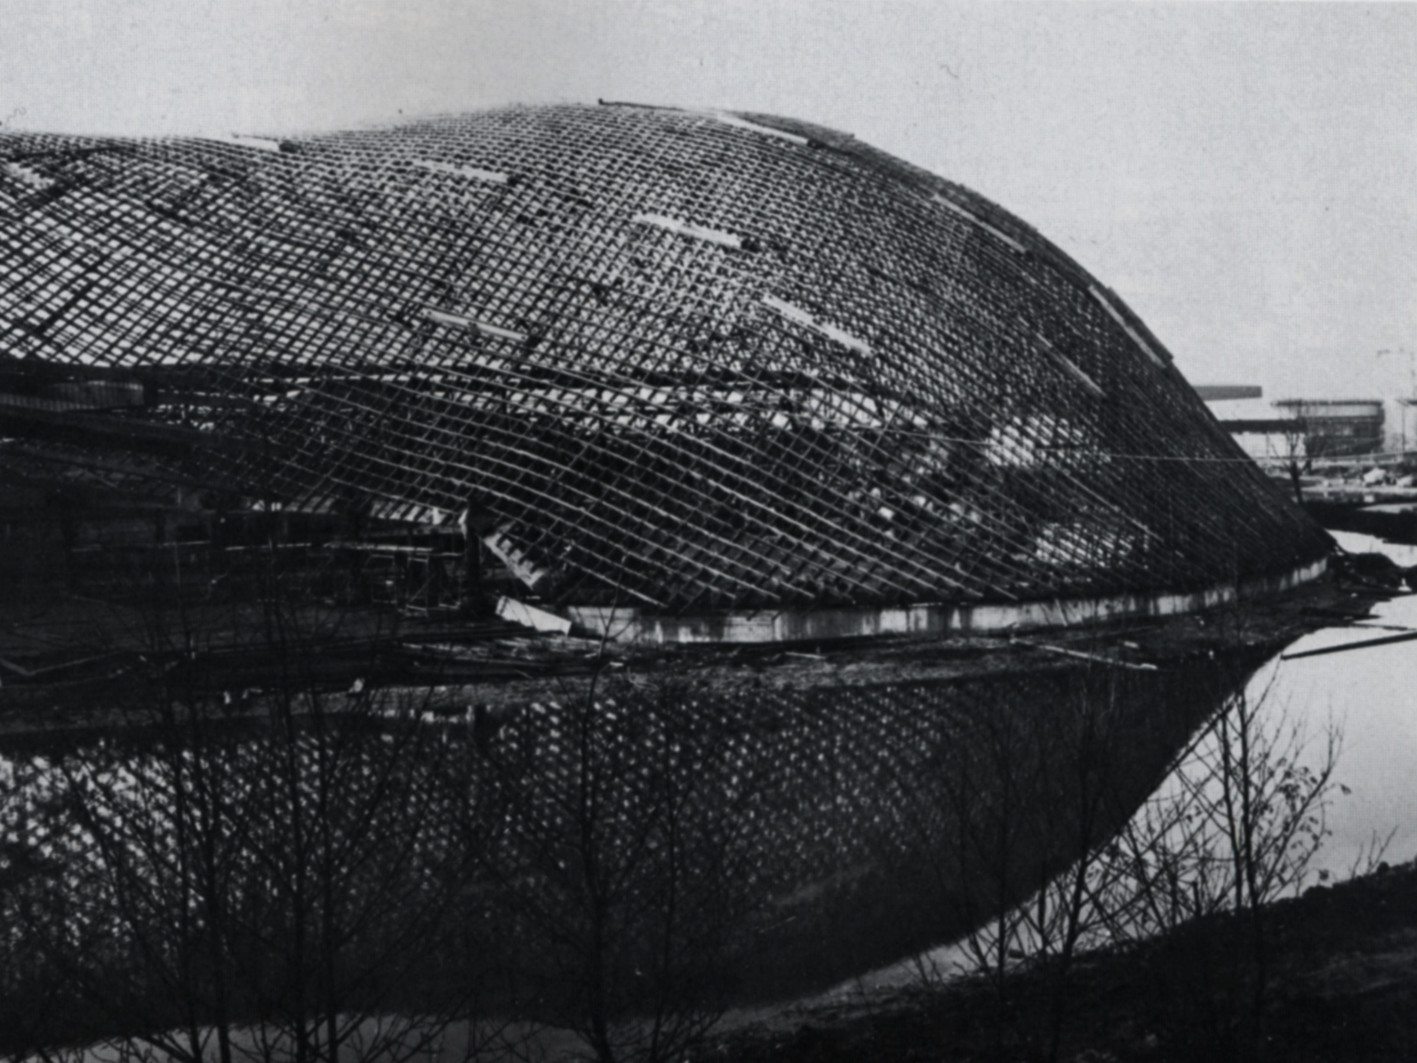
\includegraphics[width=\textwidth]{mannheim_erection_2.jpg}
			\caption{Deformed grid}
			\label{fig:erec_2}
		\end{subfigure}
		\caption[Forming process of the timber lattice of Mannheim, Germany]{Forming process of the timber lattice of Mannheim, Germany.}
		\label{fig:multihalle}
		% \hrule
	\end{figure}

	\clearpage
page 1
	\begin{tikzpicture}[remember picture,overlay, inner sep=0pt]
		\node[anchor=north east, xshift=-2cm, yshift=-2cm] at (current page.north east){
		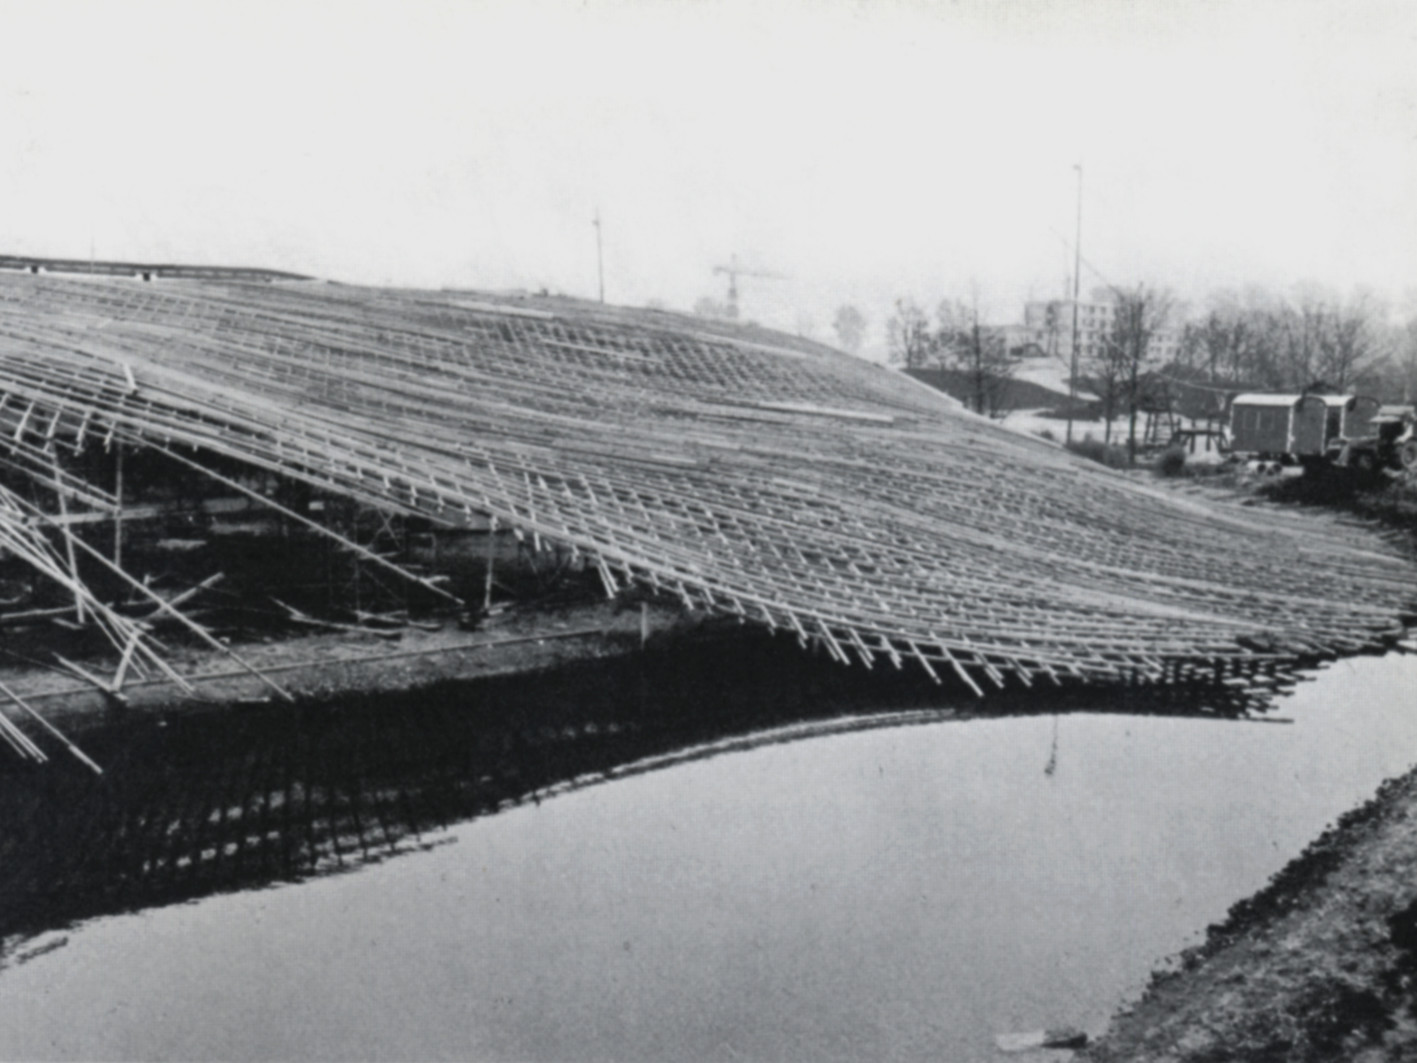
\includegraphics[width=.5\paperwidth]{mannheim_erection_1.jpg}};
		\node[anchor=north east, xshift=-2cm, yshift=-12cm] at (current page.north east){
		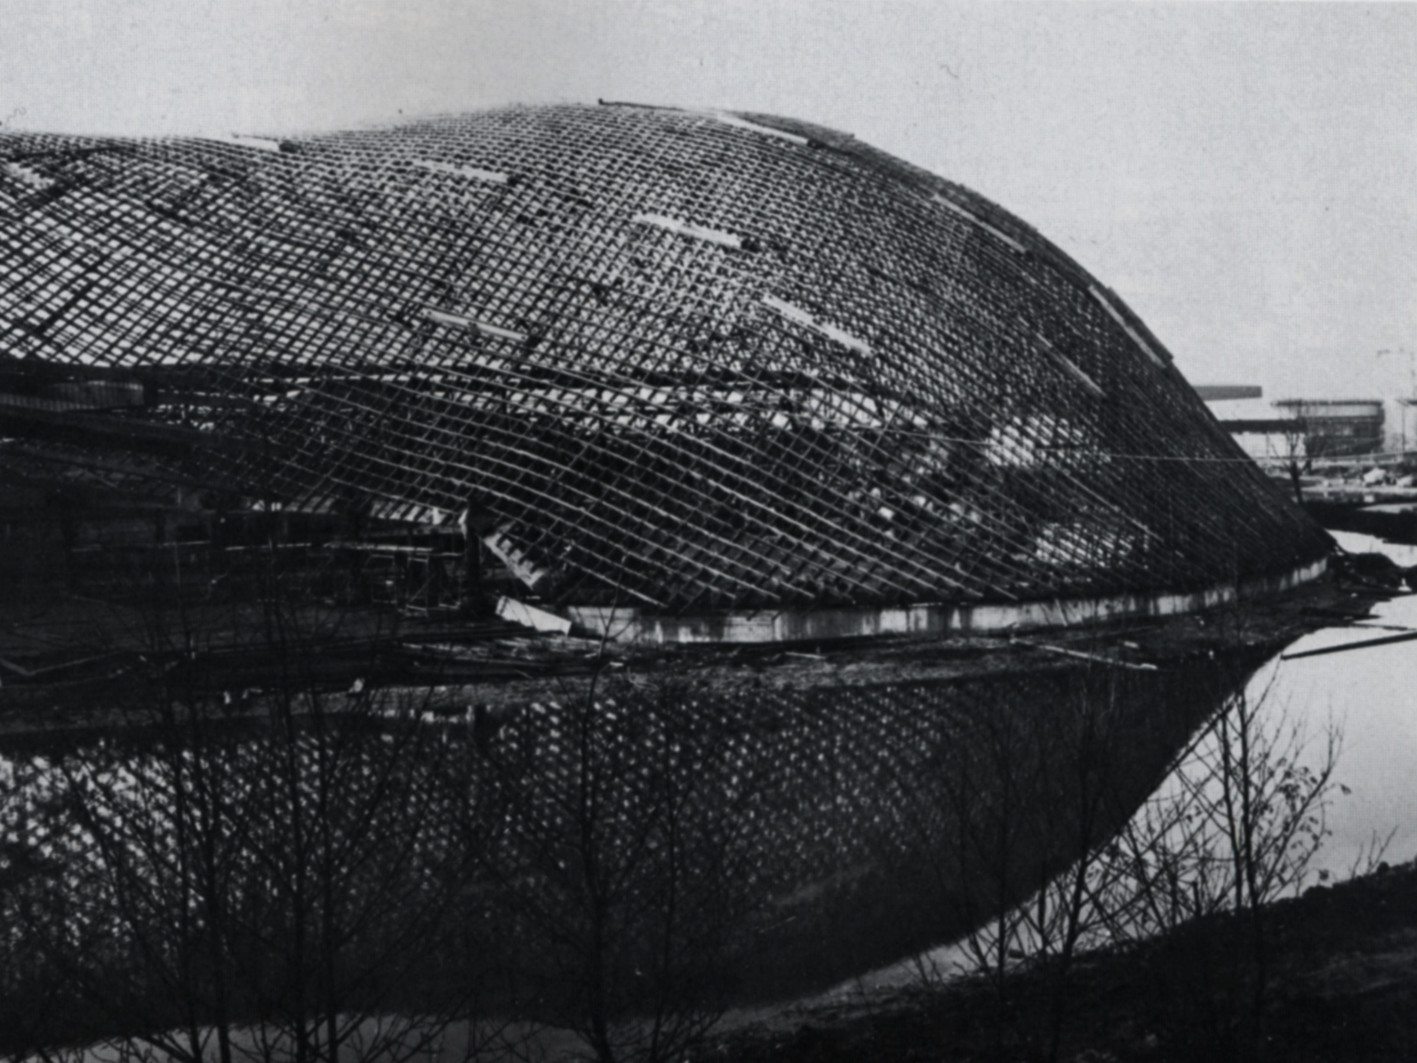
\includegraphics[width=.5\paperwidth]{mannheim_erection_2.jpg}
		};
	\end{tikzpicture}


	\clearpage
page 2
	\begin{textblock*}{5cm}(8cm,2cm)%
		\setlength{\parskip}{0pt}
		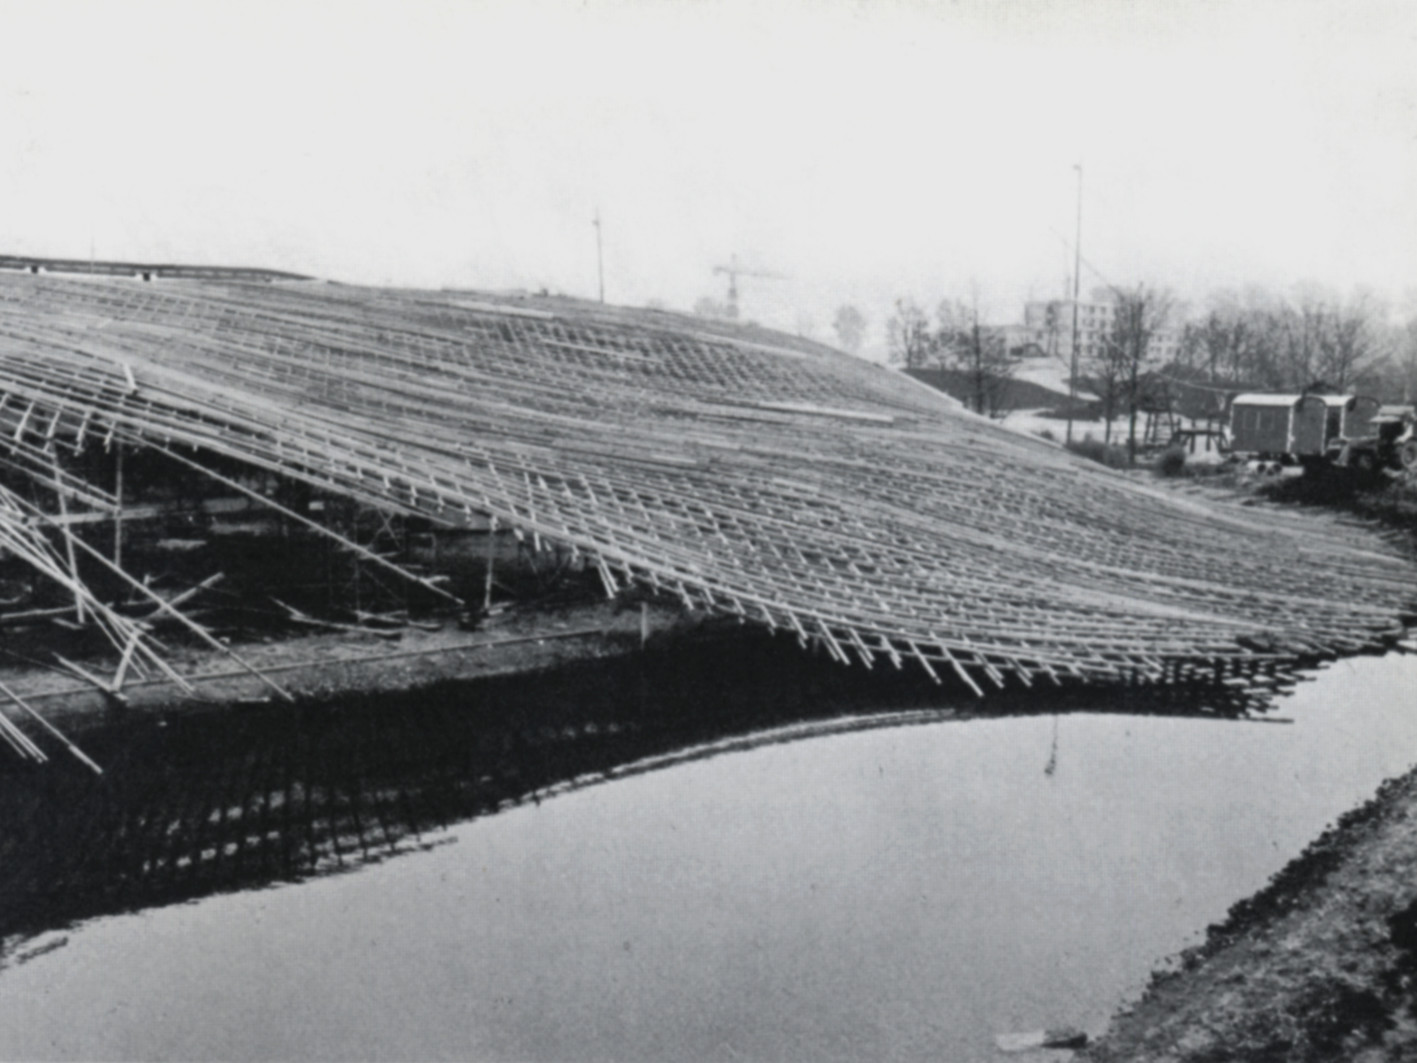
\includegraphics[width=.5\paperwidth]{mannheim_erection_1.jpg}
		\captionof{subfigure}{Mannheim\label{fig:m1}}
	\end{textblock*}
	\begin{textblock*}{5cm}(8cm,12cm)%
		\setlength{\parskip}{0pt}
		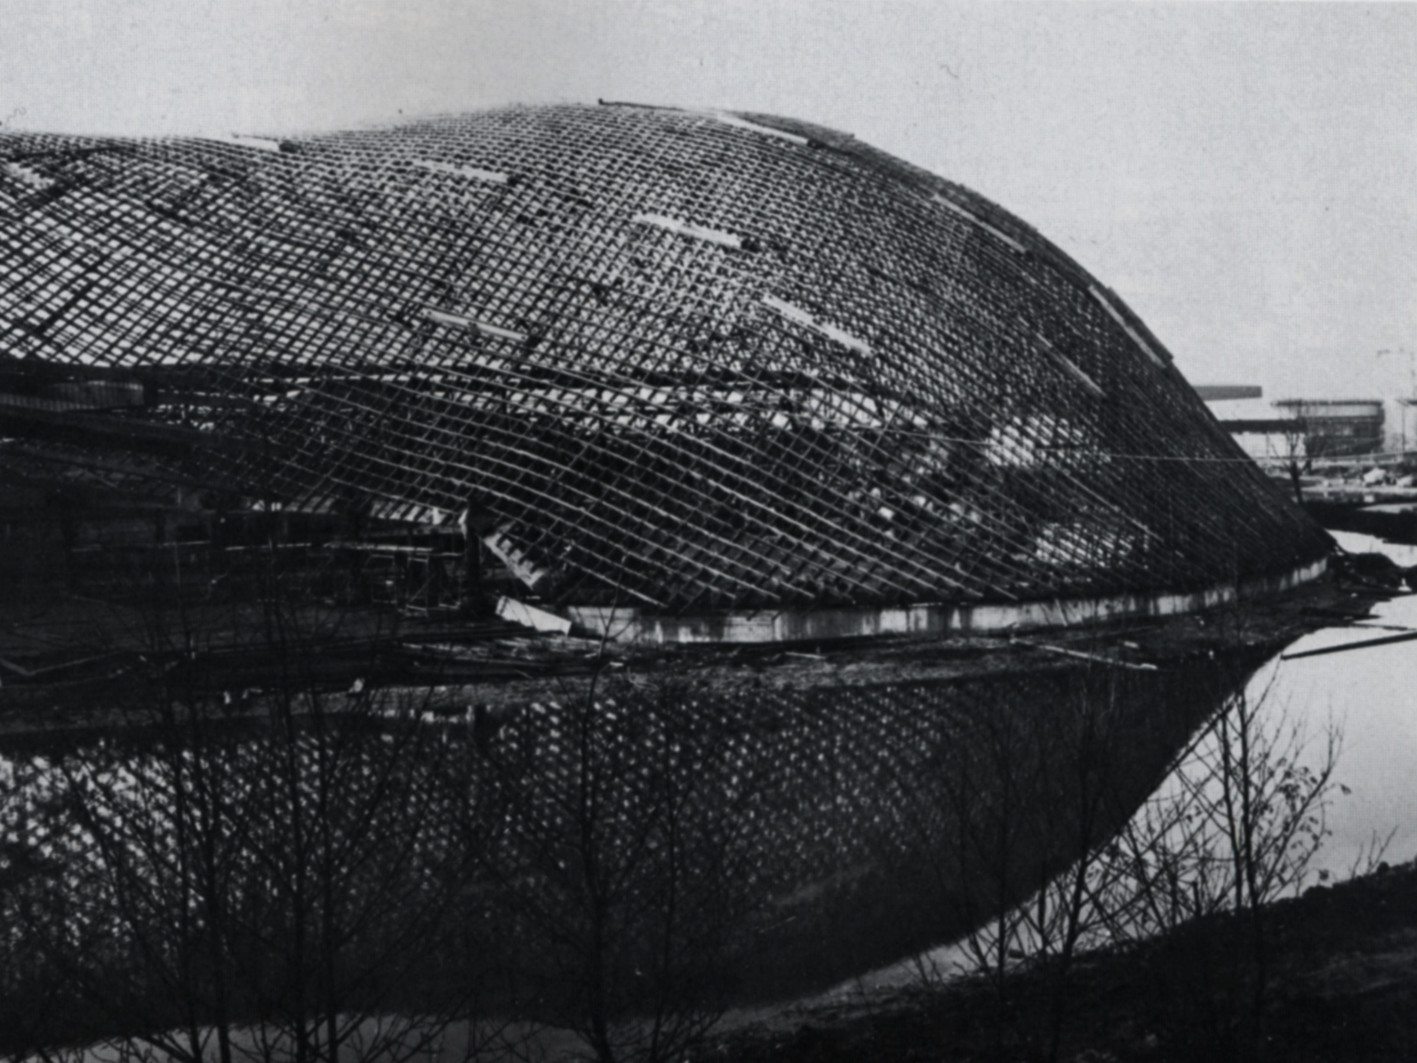
\includegraphics[width=.5\paperwidth]{mannheim_erection_2.jpg}
		\captionof{subfigure}{Mannheim\label{fig:m2}}
	\end{textblock*}



	\clearpage

	\begin{textblock*}{10cm}(0cm,0cm)%
		\setlength{\parskip}{0pt}
		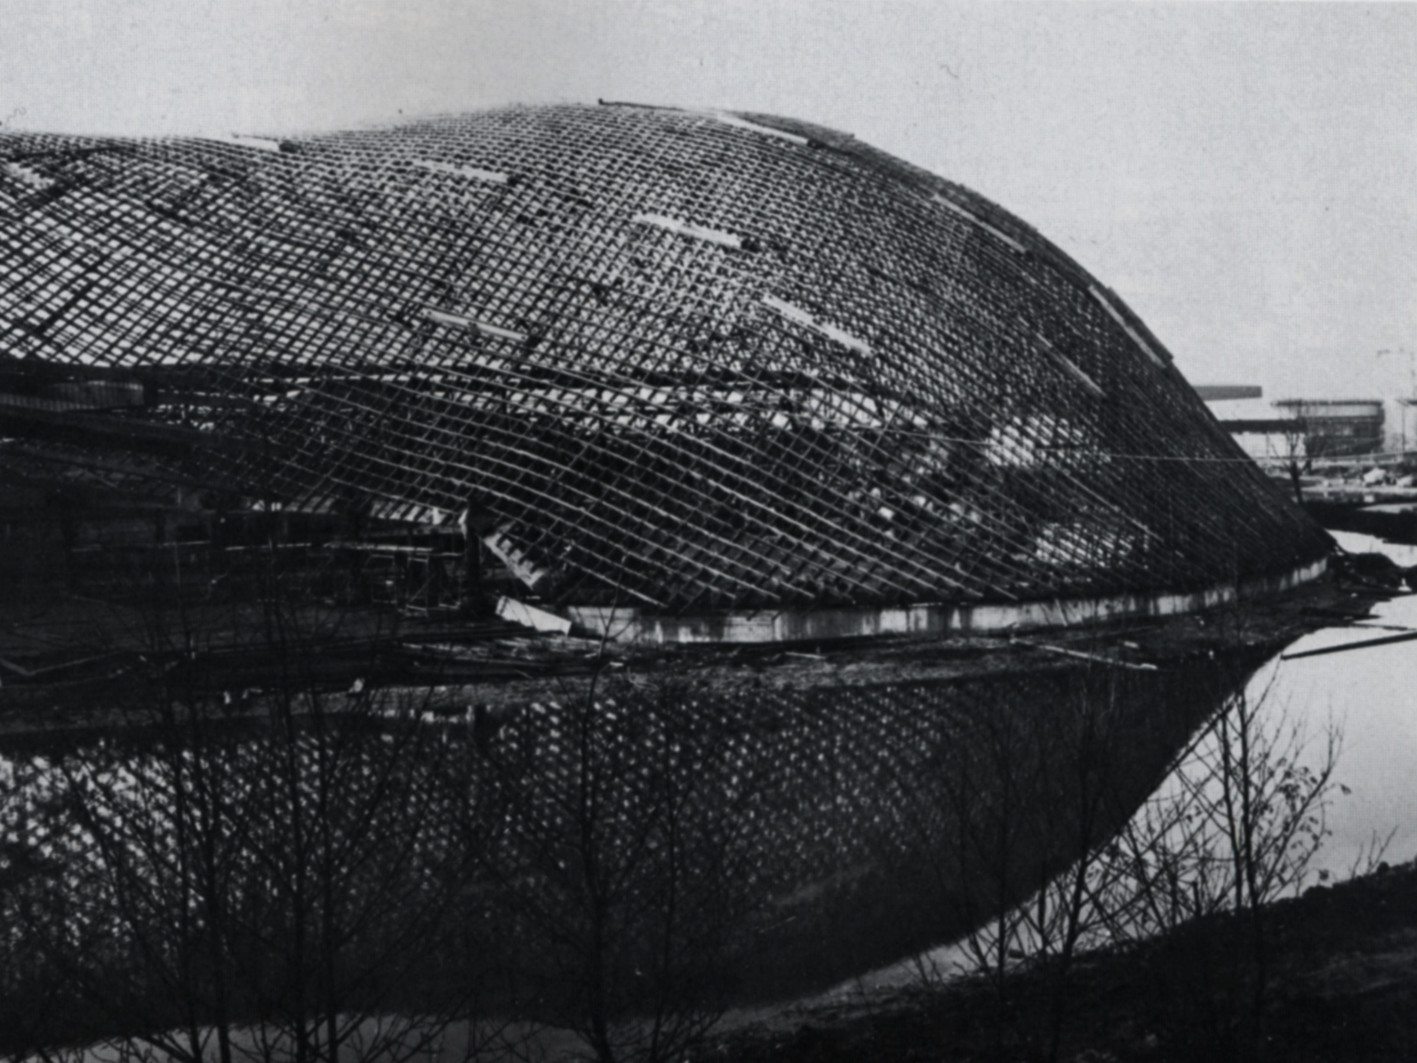
\includegraphics[width=.25\paperwidth]{mannheim_erection_2.jpg}
		\captionof{figure}{Mannheim\label{fig:twospread}}
	\end{textblock*}

	\begin{textblock*}{10cm}(0cm,14cm)%
		\setlength{\parskip}{0pt}
		\begin{figure}[t]
			\begin{subfigure}[b]{\TwoMediaWidth}
				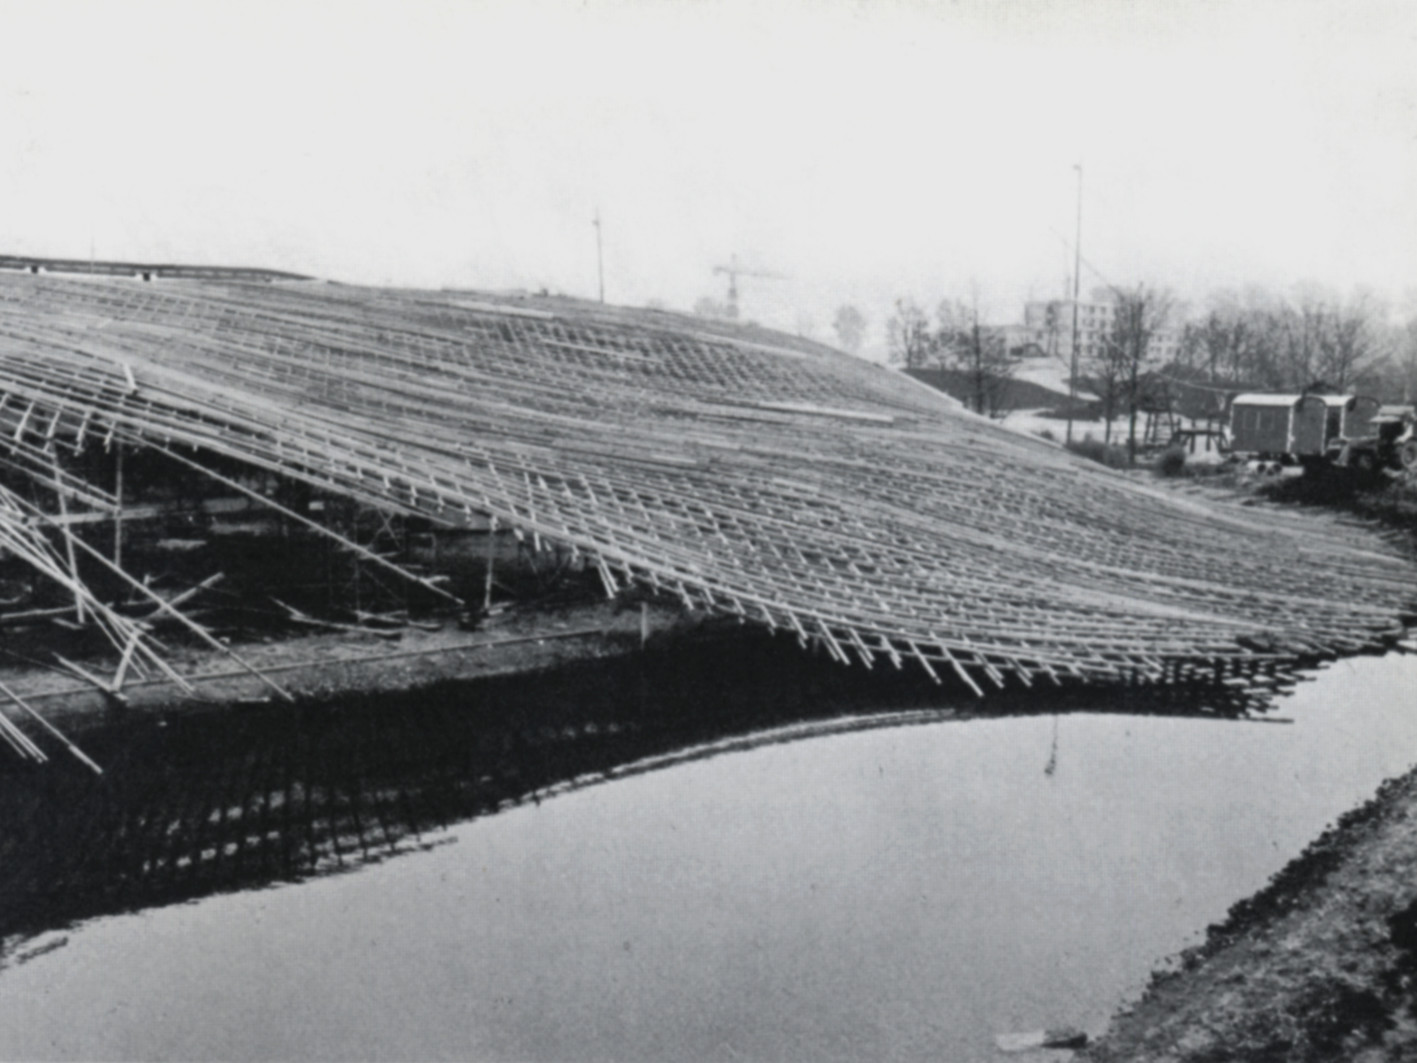
\includegraphics[width=\textwidth]{mannheim_erection_1.jpg}
				\caption{Almost flat grid}
				\label{fig:erec_1}
			\end{subfigure}%
			\hspace{\MediaGutterWidth}%
			\begin{subfigure}[b]{\TwoMediaWidth}
				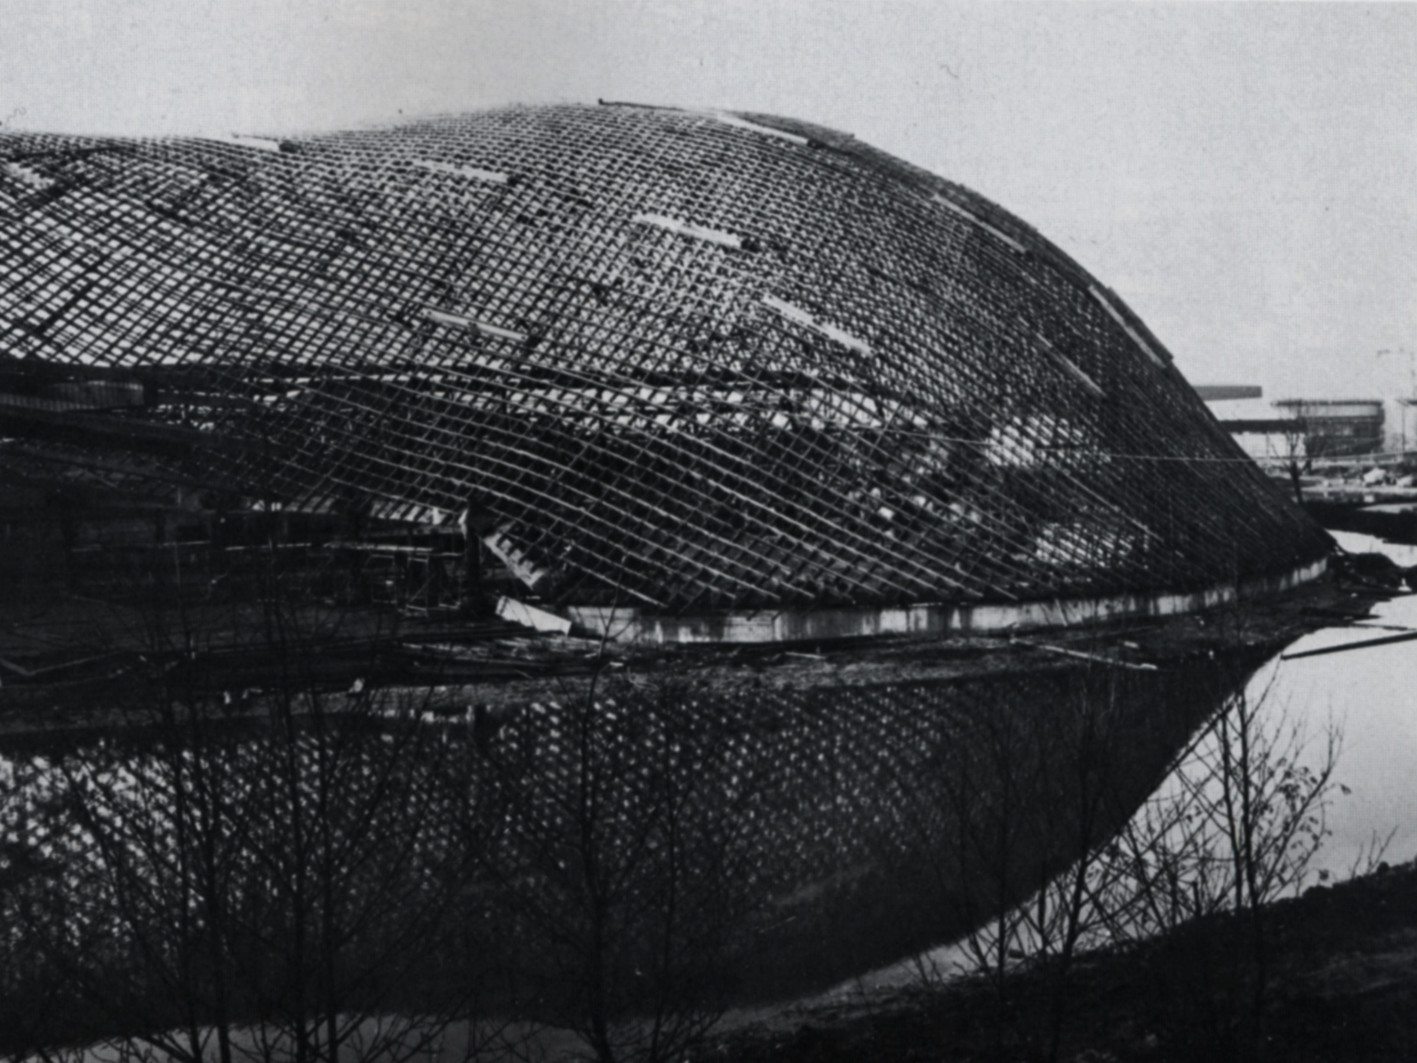
\includegraphics[width=\textwidth]{mannheim_erection_2.jpg}
				\caption{Deformed grid}
				\label{fig:erec_2}
			\end{subfigure}
			\caption[Forming process of the timber lattice of Mannheim, Germany]{Forming process of the timber lattice of Mannheim, Germany.}
			\label{fig:multihalle}
		\end{figure}
	\end{textblock*}

	% \clearpage
	% \begin{textblock*}{10cm}(10cm,16cm)%
	% 	\setlength{\parskip}{0pt}
	% 	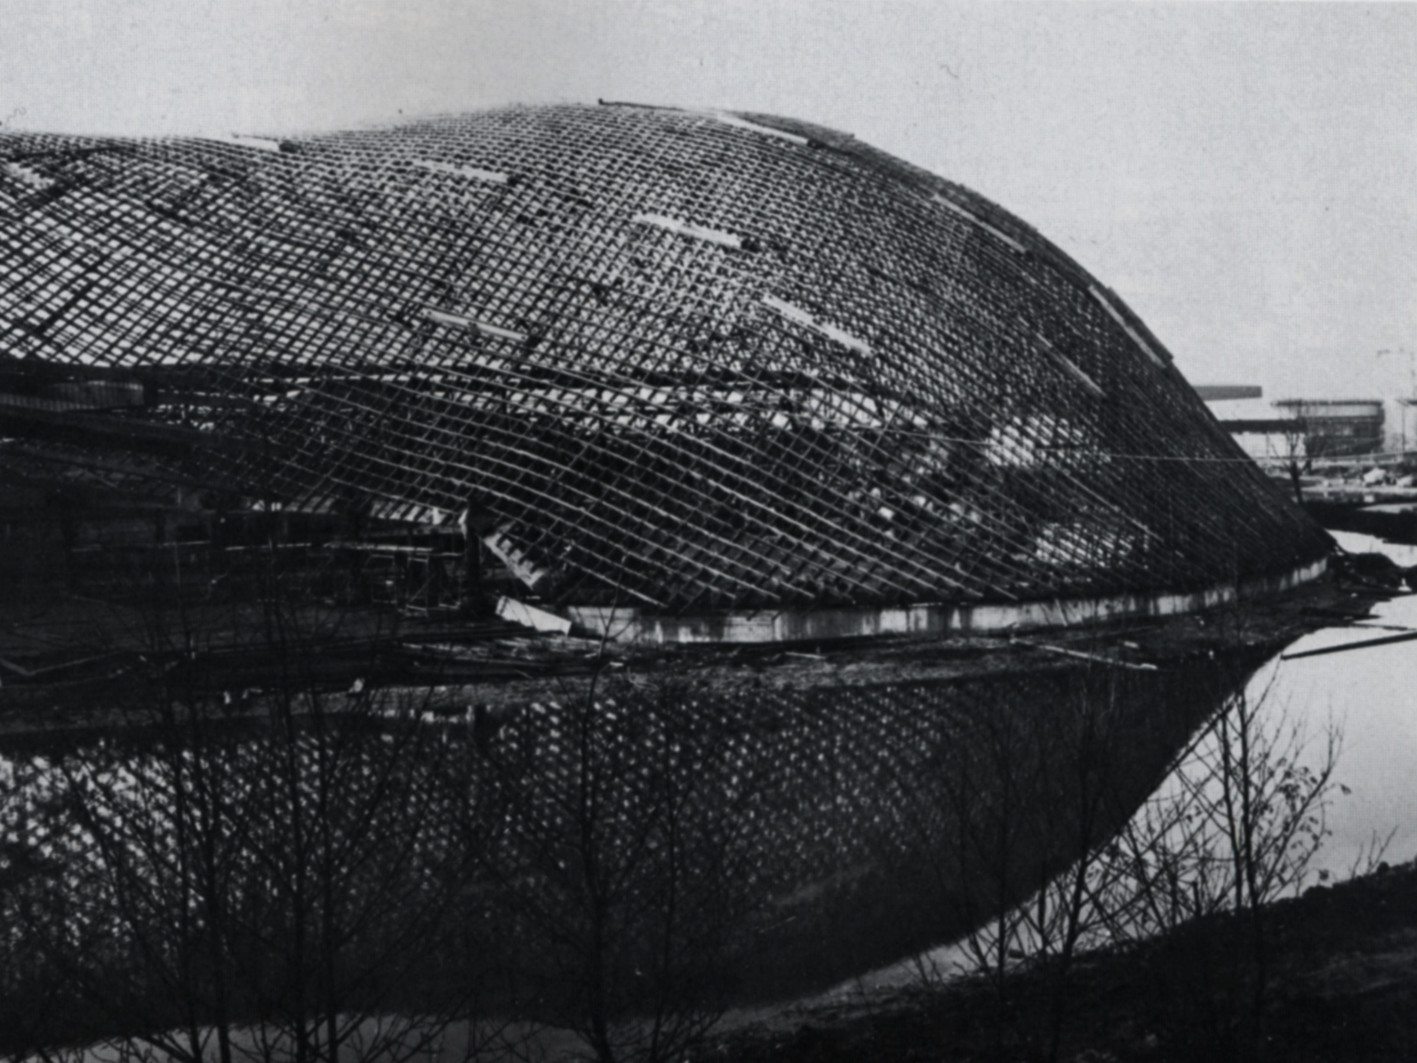
\includegraphics[width=.25\paperwidth]{mannheim_erection_2.jpg}
	% 	\captionof{figure}{Mannheim\label{fig:twospread}}
	% \end{textblock*}

	% \cleartoleftpage
	% \PhotoSpread[lpcode=\mycap]{savill_a.jpg}

	% north west
	\cleartoleftpage
	\kant[1-2]	
	\PhotoSpread[width=1.3\paperwidth,xshift=1.5cm,yshift=-1.5cm,boxcode=\mycap]{savill_a.jpg}

	% south west
	\cleartoleftpage
	\kant[1-2]	
	\PhotoSpread[yanchor=south,width=1.3\paperwidth,xshift=1cm,yshift=1cm,boxcode=\mycap]{savill_a.jpg}

	% north east
	\cleartoleftpage
	\kant[1-2]	
	\PhotoSpread[lpstyle=plain,yanchor=north,xanchor=east,width=1.3\paperwidth,xshift=-1cm,yshift=-1cm,boxcode=\mycap]{savill_a.jpg}

	% south east
	\cleartoleftpage
	\kant[1-2]	
	\PhotoSpread[lpstyle=plain,yanchor=south,xanchor=east,width=1.3\paperwidth,xshift=-1cm,yshift=1cm,boxcode=\mycap]{savill_a.jpg}


	% ==========================


	
\end{document}